%
% main.tex -- Paper zum Thema <elastomechanik>
%
% (c) 2020 Autor, OST Ostschweizer Fachhochschule
%
% !TEX root = ../../buch.tex
% !TEX encoding = UTF-8
%
\chapter{Elastomechnik – Mathematische Herleitung und ihr Weg in die ingenieurtechnische Anwendung\label{chapter:elastomechanik}}
\kopflinks{Elastomechnik}
\begin{refsection}
\chapterauthor{Sofia Aaltonen und Ricardo Rafael Barbosa Monteiro}

%
% einleitung.tex -- Beispiel-File für die Einleitung
%
% (c) 2020 Prof Dr Andreas Müller, Hochschule Rapperswil
%
% !TEX root = ../../buch.tex
% !TEX encoding = UTF-8
%

\section{Grundlagen der Fourier-Analyse\label{fourier:section:teil0}}
\kopfrechts{Teil 0}

Die Fourier-Analyse ist ein sehr mächtiges Mittel in der Signal-Analyse. 
Einleitung...


% In der Wellenfunktion gibt es keine Sprünge -> Footnote alle Fourierreihen, welche wir brauchen konvergieren.

% Wo wollen wir damit hin? Ziel klar definieren. 
% Mögliche Strategie: Hinten beginnen.
% Da schreiben; klarer, was man vorher braucht und dann schrittweise aufführen. 
% Gedanken über Schritte machen.
% Bei Wellengleichung beginnen --> Fourierreihe --> 

\subsection{Fourierreihe\label{fourier:subsection:fourierreihe}}

Mit der Fourier-Reihe lassen sich periodisch wiederholende Funktionen, wie ein Rechteck- oder Dreiecksignal, mit skalierten Sinus- und Kosinus-Schwingungen darstellen.
Um die Reihe aufzustellen, braucht man nur 3 Koeffizienten zu bestimmen. 

\begin{itemize}
	\item $a_0$ ist der Mittelwert, der Funktion. 
	Dieser entspricht dem Integral über eine Periode und schliesslich geteilt durch die Periode. 
	
	\begin{equation}
		a_0 = \frac{1}{T} \int_{t_0}^{t_0 + T} f(t) \, dx
	\end{equation}
	
	\item $a_n$ beschreibt den geraden Anteil der Funktion.
	
	\begin{equation}
		a_n = \frac{2}{T} \int_{t_0}^{t_0 + T} f(t) \cos\left(\frac{2\pi n t}{T}\right) dt
	\end{equation}
	
	\item $b_n$ beschreibt den ungeraden Anteil der Funktion.
	
	\begin{equation}
		b_n = \frac{2}{T} \int_{t_0}^{t_0 + T} f(t) \sin\left(\frac{2\pi n t}{T}\right) dt
	\end{equation}
	
\end{itemize}

Mit allen Koeffizienten bestimmt lässt sich die ursprüngliche Funktion nachahmen.
Bei Funktionen mit Sprungstellen tritt das Gibbsche Phänomen auf.
Dies erklärt einen Überschwinger nach einem Sprung. Auch wenn man die unendliche Summe bildet, wird dieser Überschwinger nicht verschwinden.
Das $=$ Zeichen stimmt also nur bedingt.
Anhand der Abbildung ... sieht man sehr schön, wie die Rechteckfunktion mit Schwingungen nachgeahmt wird.

\[
f(t) = \frac{a_0}{2} + \sum_{n=1}^{\infty} \left( a_n \cos\left( \frac{2\pi n}{T} x \right) + b_n \sin\left( \frac{2\pi n}{T} x \right) \right)
\]

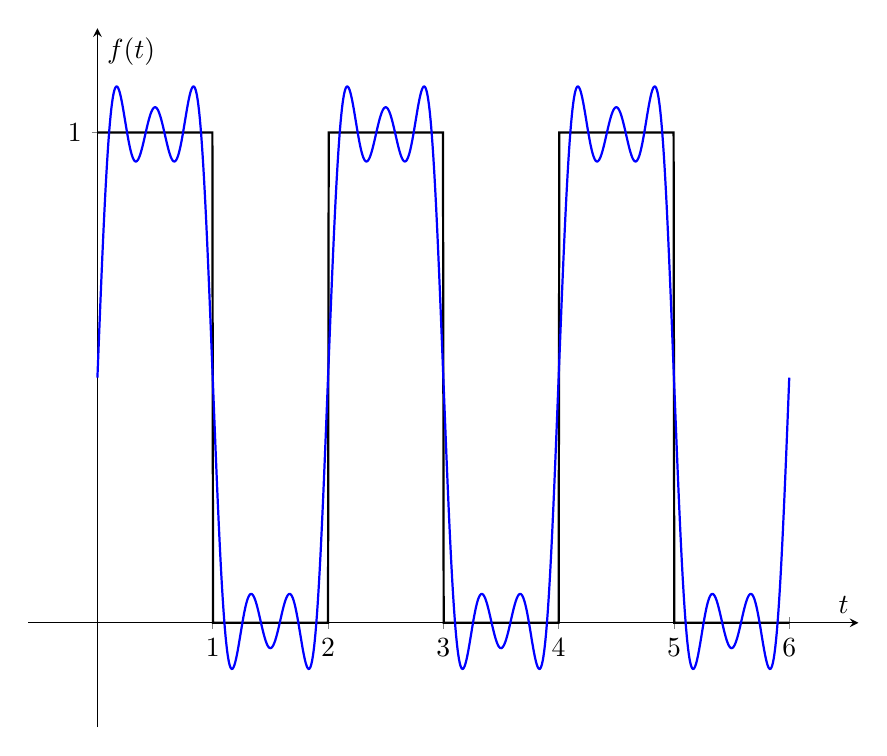
\begin{tikzpicture}
	\begin{axis}[
		axis lines = middle,
		xlabel = {$t$},
		ylabel = {$f(t)$},		
		domain=0:6,
		samples=1000,
		xtick={0,1,2,3,4,5,6},
		ytick={0,1},
		enlargelimits,
		width=\textwidth
		]
		\addplot[thick] {mod(floor(x),2) == 0 ? 1 : 0};
		\addplot[blue, thick] {(1/2) + 
			(2/pi)*sin(pi * deg(x)) + 
			(2/(3*pi))*sin(pi *3*deg(x)) +
			(2/(5*pi))*sin(pi *5*deg(x))};
	\end{axis}
\end{tikzpicture}

$a_0$ ist bei 


\subsection{Fouriertransformation\label{fourier:subsection:fouriertransformation}}


%
% teil1.tex -- Beispiel-File für das Paper
%
% (c) 2020 Prof Dr Andreas Müller, Hochschule Rapperswil
%
% !TEX root = ../../buch.tex
% !TEX encoding = UTF-8
%
\section{Metrik und Hodge-Theorie 
\label{maxwell:section:teil1}}
\kopfrechts{Metrik und Hodge-Theorie}

\subsection{Minkowski Metrik}
In der speziellen Relativitätstheorie (SRT) wird die Minkowski-Metrik verwendet.
\index{spezielle Relativitätstheorie}%
\index{Relativitätstheorie, spezielle}%
\index{Minkowski-Metrik}%
Da es in der SRT keine Krümmung und Gravitation gibt, sind alle Elemente ausserhalb der Diagonale des metrischen Tensors null und somit ist die Raum-Zeit flach.
Zwei Signaturen sind üblich.
Einerseits gibt es die $({-}{+}{+}{+})$-Signatur, bei welcher die Zeitkomponente negativ und die Raumkomponenten positiv gezählt werden.
Andererseits gibt es die $({+}{-}{-}{-})$-Signatur, bei welcher die Zeitkomponente positiv und die Raumkomponenten negativ gezählt werden.
Beide Signaturen sind gleichwertig, solange man sich auf eine Metrik festlegt und diese konsequent beibehält.
Im Folgenden werden wir uns an die $({-}{+}{+}{+})$-Signatur halten.
Daher definieren wir den metrischen Tensor als
\begin{equation}
	g^{ik} = \begin{pmatrix}
		-1 & 0 & 0 & 0 \\ 0 & 1 & 0 & 0 \\ 0 & 0 & 1 & 0 \\ 0 & 0 & 0 & 1 
	\end{pmatrix}.
	\label{maxwell:section:teil1:metrik}
\end{equation}
Der Ausdruck für ein Linienelement in dieser Metrik ist definiert als
\begin{equation*}
	dl^2 = -(dx^0)^2 +(dx^1)^2+(dx^2)^2+(dx^3)^2.
\end{equation*}
Damit wir Raum und Zeit in dieser Metrik gleichartig behandeln können, wählen wir beim Übergang in physikalische Einheiten 
\begin{equation}
	\label{maxwell:koordinaten}
	x^0 = ct,\quad x^1 = x,\quad x^2 = y, \quad x^3 = z .
\end{equation}
Dabei entspricht $c$ der Lichtgeschwindigkeit und ein Linienelement ist somit definiert als
\begin{equation*}
	dl^2 = -c^2dt^2 +dx^2+dy^2+dz^2.
\end{equation*}
Eine Konsequenz dieser Signatur ist, dass zeitartige Abstände $dl^2 < 0$ und raumartige Abstände $dl^2 > 0$ sind.

\subsection{Hodge-Duale der Basis-$k$-Formen}
Für den Teil der inhomogenen Maxwell-Gleichungen benötigen wir die Hodge-Duale von 1-Formen, 2-Formen und 3-Formen im vierdimensionalen Minkowski-Raum.
Um dabei die korrekten Vorzeichen zu erhalten, muss die Hodge-Dualität mit Hilfe des metrischen Tensors $g^{ik}$  der Minkowski-Metrik verwendet werden.

Wir verwenden die Definition des Hodge-Operators
\begin{equation*}
	\alpha \wedge \ast \beta = \langle \alpha, \beta \rangle \operatorname{vol}(M),
\end{equation*}
wobei $\langle \cdot , \cdot \rangle$ das durch die Metrik $g^{ik}$ induzierte Skalarprodukt ist.
Im Folgenden führen wir alle Berechnungen der Hodge-Duale von 1-, 2- und 3-Formen durch.
Wir verwenden $g^{ik}$ gemäss \eqref{maxwell:section:teil1:metrik} und $\operatorname{vol}(M) = dx^0 \wedge dx^1 \wedge dx^2 \wedge dx^3$.
\begin{definition}
\label{maxwell:hodge:kurzschreibweise}
Um die Notation kompakter und übersichtlicher zu gestalten, führen wir die Schreibweise
\begin{align*}
	dx^{i\!j} &:= dx^i \wedge dx^j, 
	%\label{maxwell:hodge:zwei}
	\\
	dx^{i\!jk} &:= dx^i \wedge dx^j \wedge dx^k, 
	%\label{maxwell:hodge:drei}
	\\
	dx^{i\!jkl} & := dx^i \wedge dx^j \wedge dx^k \wedge dx^l
	\notag
\end{align*}
für Wedge-Produkte von Basisformen ein.
\end{definition}
Mit dieser Vorbereitung können wir nun die konkreten Hodge-Duale der Basisformen berechnen.
\subsubsection{Hodge-Duale von 1-Formen}
\begin{align*}
	\ast dx^0 
	&= s \, dx^{123} \\
	dx^0 \wedge \ast dx^0 
	&= dx^0 \wedge s \, dx^{123} = s \, dx^{0123} \\
	&= \langle dx^0, dx^0 \rangle \operatorname{vol}(M) = g^{00} \, dx^{0123} = -dx^{0123} \\
	\Rightarrow s &= -1 \Rightarrow \boxed{\ast dx^0 = - dx^{123}}
	\\[1em]
	\ast dx^1 
	&= s \, dx^{023} \\
	dx^1 \wedge \ast dx^1 
	&= dx^1 \wedge s \, dx^{023} = -s \, dx^{0123} \\
	&= \langle dx^1, dx^1 \rangle \operatorname{vol}(M) = g^{11} \, dx^{0123} = dx^{0123} \\
	\Rightarrow s &= -1 \Rightarrow \boxed{\ast dx^1 = - dx^{023}}
	\\[1em]
	\ast dx^2 
	&= s \, dx^{013} \\
	dx^2 \wedge \ast dx^2 
	&= dx^2 \wedge s \, dx^{013} = s \, dx^{0123} \\
	&= \langle dx^2, dx^2 \rangle \operatorname{vol}(M) = g^{22} \, dx^{0123} = dx^{0123} \\
	\Rightarrow s &= +1 \Rightarrow \boxed{\ast dx^2 = dx^{013}}
	\\[1em]
	\ast dx^3 
	&= s \, dx^{012} \\
	dx^3 \wedge \ast dx^3 
	&= dx^3 \wedge s \, dx^{012} = -s \, dx^{0123} \\
	&= \langle dx^3, dx^3 \rangle \operatorname{vol}(M) = g^{33} \, dx^{0123} = dx^{0123} \\
	\Rightarrow s &= -1 \Rightarrow \boxed{\ast dx^3 = - dx^{012}}
\end{align*}

\subsubsection{Hodge-Duale von 2-Formen}
\begin{align*}
	\ast dx^{01} &= s \, dx^{23} \\
	dx^{01} \wedge \ast dx^{01} &= s \, dx^{0123} \\
	&= \langle dx^{01}, dx^{01} \rangle \, \operatorname{vol}(M) 
	= g^{00} g^{11} \operatorname{vol}(M) = -dx^{0123} \\
	\Rightarrow s &= -1 \Rightarrow \boxed{\ast dx^{01} = - dx^{23}}
	\\[1em]
	\ast dx^{12} &= s \, dx^{03} \\
	dx^{12} \wedge \ast dx^{12} &= s \, dx^{0123} \\
	&= \langle dx^{12}, dx^{12} \rangle \, \operatorname{vol}(M) 
	= g^{11} g^{22} \operatorname{vol}(M) = dx^{0123} \\
	\Rightarrow s &= +1 \Rightarrow \boxed{\ast dx^{12} = dx^{03}}
	\\[1em]
	\ast dx^{23} &= s \, dx^{01} \\
	dx^{23} \wedge \ast dx^{23} &= s \, dx^{0123} \\
	&= \langle dx^{23}, dx^{23} \rangle \, \operatorname{vol}(M) 
	= g^{22} g^{33} \operatorname{vol}(M) = dx^{0123} \\
	\Rightarrow s &= +1 \Rightarrow \boxed{\ast dx^{23} = dx^{01}}
	\\[1em]
	\ast dx^{02} &= s \, dx^{13} \\
	dx^{02} \wedge \ast dx^{02} &= -s \, dx^{0123} \\
	&= \langle dx^{02}, dx^{02} \rangle \, \operatorname{vol}(M) 
	= g^{00} g^{22} \operatorname{vol}(M) = -dx^{0123} \\
	\Rightarrow s &= +1 \Rightarrow \boxed{\ast dx^{02} = dx^{13}}
	\\[1em]
	\ast dx^{03} &= s \, dx^{12} \\
	dx^{03} \wedge \ast dx^{03} &= s \, dx^{0123} \\
	&= \langle dx^{03}, dx^{03} \rangle \, \operatorname{vol}(M) 
	= g^{00} g^{33} \operatorname{vol}(M) = -dx^{0123} \\
	\Rightarrow s &= -1 \Rightarrow \boxed{\ast dx^{03} = - dx^{12}}
	\\[1em]
	\ast dx^{13} &= s \, dx^{02} \\
	dx^{13} \wedge \ast dx^{13} &= -s \, dx^{0123} \\
	&= \langle dx^{13}, dx^{13} \rangle \, \operatorname{vol}(M) 
	= g^{11} g^{33} \operatorname{vol}(M) = dx^{0123} \\
	\Rightarrow s &= -1 \Rightarrow \boxed{\ast dx^{13} = - dx^{02}}
\end{align*}

\subsubsection{Hodge-Duale von 3-Formen}
\begin{align*}
	\ast dx^{012} &= s \, dx^3 \\
	dx^{012} \wedge \ast dx^{012} &= s \, dx^{0123} \\
	&= \langle dx^{012}, dx^{012} \rangle \, \operatorname{vol}(M) 
	= g^{00} g^{11} g^{22} \operatorname{vol}(M) = -dx^{0123} \\
	\Rightarrow s &= -1 \Rightarrow \boxed{\ast dx^{012} = - dx^3}
	\\[1em]
	\ast dx^{013} &= s \, dx^2 \\
	dx^{013} \wedge \ast dx^{013} &= -s \, dx^{0123} \\
	&= \langle dx^{013}, dx^{013} \rangle \, \operatorname{vol}(M) 
	= g^{00} g^{11} g^{33} \operatorname{vol}(M) = -dx^{0123} \\
	\Rightarrow s &= 1 \Rightarrow \boxed{\ast dx^{013} = dx^2}
	\\[1em]
	\ast dx^{023} &= s \, dx^1 \\
	dx^{023} \wedge \ast dx^{023} &= s \, dx^{0123} \\
	&= \langle dx^{023}, dx^{023} \rangle \, \operatorname{vol}(M) 
	= g^{00} g^{22} g^{33} \operatorname{vol}(M) = -dx^{0123} \\
	\Rightarrow s &= -1 \Rightarrow \boxed{\ast dx^{023} = - dx^1}
	\\[1em]
	\ast dx^{123} &= s \, dx^0 \\
	dx^{123} \wedge \ast dx^{123} &= -s \, dx^{0123} \\
	&= \langle dx^{123}, dx^{123} \rangle \, \operatorname{vol}(M)
	= g^{11} g^{22} g^{33} \operatorname{vol}(M) = dx^{0123} \\
	\Rightarrow s &= -1 \Rightarrow \boxed{\ast dx^{123} = - dx^0}
\end{align*}
In der Tabelle \ref{maxwell:section:teil1:Hodge-Tabelle} sind alle berechneten Hodge-Duale noch einmal zusammengefasst.
\begin{table}
	\centering
	%\caption{Hodge-Duale}
	%\label{maxwell:section:teil1:Hodge-Tabelle}
	\begin{tabularx}{\textwidth}{ 
			| >{\centering\arraybackslash}X 
			| >{\centering\arraybackslash}X 
			| >{\centering\arraybackslash}X | }
		\hline
		\textbf{1-Form} & \textbf{2-Form} & \textbf{3-Form} \\
		\hline
		\( \rule{0pt}{1.5em} {\ast} dx^0 = -dx^1 \wedge dx^2 \wedge dx^3 \) \newline
	\( {\ast} dx^1 = -dx^0 \wedge dx^2 \wedge dx^3 \) \newline
	\( {\ast} dx^2 = \phantom{-} dx^0 \wedge dx^1 \wedge dx^3 \) \newline
	\( {\ast} dx^3 = -dx^0 \wedge dx^1 \wedge dx^2 \, \) 
	&
	\( \rule{0pt}{1.5em} {\ast} (dx^0 \wedge dx^1) = -dx^2 \wedge dx^3 \) \newline
	\( {\ast} (dx^1 \wedge dx^2) = \phantom{-} dx^0 \wedge dx^3 \) \newline
	\( {\ast} (dx^2 \wedge dx^3) = \phantom{-} dx^0 \wedge dx^1 \) \newline
	\( {\ast} (dx^0 \wedge dx^2) = \phantom{-} dx^1 \wedge dx^3 \) \newline
	\( {\ast} (dx^0 \wedge dx^3) = -dx^1 \wedge dx^2 \) \newline
	\( {\ast} (dx^1 \wedge dx^3) = -dx^0 \wedge dx^2 \)
	&
	\( \rule{0pt}{1.5em} {\ast} (dx^0 \wedge dx^1 \wedge dx^2) = -dx^3 \) \newline
	\( {\ast} (dx^0 \wedge dx^1 \wedge dx^3) = \phantom{-} dx^2 \) \newline
	\( {\ast} (dx^0 \wedge dx^2 \wedge dx^3) = -dx^1 \) \newline
	\( {\ast} (dx^1 \wedge dx^2 \wedge dx^3) = -dx^0 \)
		\\
		\hline
	\end{tabularx}
	\caption{Tabelle aller Hodge-Duale von 1-, 2-, und 3-Formen mit $({-}{+}{+}{+})$-Signatur}
	\label{maxwell:section:teil1:Hodge-Tabelle}
\end{table}








%
% teil2.tex -- Beispiel-File für teil2 
%
% (c) 2020 Prof Dr Andreas Müller, Hochschule Rapperswil
%
% !TEX root = ../../buch.tex
% !TEX encoding = UTF-8
%
\section{Vorgeschriebene gausssche Krümmung
\label{mongeampere:section:teil2}}
\kopfrechts{Teil 2}
Mit der Definition der gausschen Krümmung können wir nun eine Differentialgleichung aufstellen,
welche als Lösung eine Fläche mit einer gewünschten gausschen Krümmung hat.
Dafür nehmen wir die explizite Form einer Fläche $z = f(x,y)$.
Die Variablen sind nun nicht mehr $u, v$ sondern $x, y$.
Nun brauchen wir die Koeffizienten der Fundamentalformen, welche mit dem Radiusvektor $\vec r$ und seinen Ableitungen 
beschrieben werden können
\begin{align}
  \vec r &= \begin{pmatrix}
   x \\
   y \\
   f(x, y)
 \end{pmatrix} \\
    \vec r_x &= \begin{pmatrix}
      1 \\
      0 \\
      \frac{\partial f}{\partial x}
    \end{pmatrix},
      \quad &
    \vec r_y &= \begin{pmatrix}
      0 \\
      1 \\
      \frac{\partial f}{\partial y}
    \end{pmatrix}\\
      \vec r_{xx} &= \begin{pmatrix}
      0 \\
      0 \\
      \frac{\partial^2 f}{\partial x^2}
    \end{pmatrix},
    \quad &
    \vec r_{xy} &= \begin{pmatrix}
      0 \\
      0 \\
      \frac{\partial^2 f}{\partial x \, \partial y}
    \end{pmatrix},
      \quad &
    \vec r_{yy} &= \begin{pmatrix}
      0 \\
      0 \\
      \frac{\partial^2 f}{\partial y^2}
    \end{pmatrix}\\
\end{align}
Damit sind die Koeffizienten der ersten Fundamentalform 
\begin{equation}
  E = 1 + \left(\frac{\partial f}{\partial x}\right)^2, \quad
  F = \frac{\partial f}{\partial x} \cdot \frac{\partial f}{\partial y}, \quad
  G = 1 + \left(\frac{\partial f}{\partial y}\right)^2
  \label{mongeampere:fund1exp}
\end{equation}
Für die zweite Fundamentalform wird die Flächennormale benötigt, welche aus \eqref{mongeampere:norm} und \eqref{mongeampere:ds} 
\begin{equation}
  \vec m = \frac{\vec r_x \times \vec r_y}{\sqrt{EG-F^2}} = \begin{pmatrix}
    \frac{\partial f}{\partial x} \\
    \frac{\partial f}{\partial y} \\
    1
  \end{pmatrix}
  \frac{1}{\sqrt{EG-F^2}}
  \label{mongeampere:norm2}
\end{equation}
ist.
Somit sind die Koeffizienten der zweiten Fundamentalform
\begin{equation}
  L = \frac{\frac{\partial^2 f}{\partial x^2}}{\sqrt{EG-F}}, \quad
  M = \frac{\frac{\partial^2 f}{\partial x \, \partial y}}{\sqrt{EG-F}}, \quad
  N = \frac{\frac{\partial^2 f}{\partial y^2}}{\sqrt{EG-F}}
  \label{mongeampere:2fund22}
\end{equation}
Setzen wir die Koeffizienten aus \eqref{mongeampere:fund1exp} und \eqref{mongeampere:2fund22} in die Formel der gausschen Krümmung \eqref{mongeampere:gausskrumm}
ein, erhalten wir
\begin{equation}
  K = \frac{
    \frac{\partial^2 f}{\partial x^2} \cdot \frac{\partial^2 f}{\partial y^2} - \left(\frac{\partial^2 f}{\partial x \, \partial y} \right)^2}
    {\left[1 + 
    \left(\frac{\partial f}{\partial x}\right)^2 +
    \left(\frac{\partial f}{\partial y}\right)^2\right]^2}.
  \label{mongeampere:pd}
\end{equation}
Wie wir sehen können, ist der Zähler gleich der Determinante der hesseschen Matrix von $f(x,y)$.
Der Nenner ist eine nichtlineare Funktion der ersten Ableitungen.
Somit konnten wir zeigen, dass das Prescribed Gaussian Curvature Problem einer explizit definierten Fläche in einer 
monge-ampèreschen Gleichung resultiert.


%
% teil3.tex -- Beispiel-File für Teil 3
%
% (c) 2020 Prof Dr Andreas Müller, Hochschule Rapperswil
%
% !TEX root = ../../buch.tex
% !TEX encoding = UTF-8
%
\section{Teil 3
\label{ueberschall:section:teil3}}
\kopfrechts{Teil 3}
Sed ut perspiciatis unde omnis iste natus error sit voluptatem
accusantium doloremque laudantium, totam rem aperiam, eaque ipsa
quae ab illo inventore veritatis et quasi architecto beatae vitae
dicta sunt explicabo. Nemo enim ipsam voluptatem quia voluptas sit
aspernatur aut odit aut fugit, sed quia consequuntur magni dolores
eos qui ratione voluptatem sequi nesciunt. Neque porro quisquam
est, qui dolorem ipsum quia dolor sit amet, consectetur, adipisci
velit, sed quia non numquam eius modi tempora incidunt ut labore
et dolore magnam aliquam quaerat voluptatem. Ut enim ad minima
veniam, quis nostrum exercitationem ullam corporis suscipit laboriosam,
nisi ut aliquid ex ea commodi consequatur? Quis autem vel eum iure
reprehenderit qui in ea voluptate velit esse quam nihil molestiae
consequatur, vel illum qui dolorem eum fugiat quo voluptas nulla
pariatur?

\subsection{De finibus bonorum et malorum
\label{ueberschall:subsection:malorum}}
At vero eos et accusamus et iusto odio dignissimos ducimus qui
blanditiis praesentium voluptatum deleniti atque corrupti quos
dolores et quas molestias excepturi sint occaecati cupiditate non
provident, similique sunt in culpa qui officia deserunt mollitia
animi, id est laborum et dolorum fuga. Et harum quidem rerum facilis
est et expedita distinctio. Nam libero tempore, cum soluta nobis
est eligendi optio cumque nihil impedit quo minus id quod maxime
placeat facere possimus, omnis voluptas assumenda est, omnis dolor
repellendus. Temporibus autem quibusdam et aut officiis debitis aut
rerum necessitatibus saepe eveniet ut et voluptates repudiandae
sint et molestiae non recusandae. Itaque earum rerum hic tenetur a
sapiente delectus, ut aut reiciendis voluptatibus maiores alias
consequatur aut perferendis doloribus asperiores repellat.



\section{Überschallknall: Entstehung und Low-Boom-Strategien
\label{schall:section:boom}}
\kopfrechts{Überschallknall: Entstehung und Low-Boom-Strategien}

In diesem Kapitel betrachten wir, warum Überschallflugzeuge am Boden
einen lauten Knall verursachen, wie sich dieser ausbreitet, und welche
Strategien es gibt, um den Knall zu reduzieren.

Ein Flugzeug mit Machzahl $\textit{Ma}\ge1$ erzeugt entlang seiner Länge diskrete
Schockbeiträge an Bug, Tragflächen, Rumpfänderungen, Leitwerke und Auspuff,
die sich bei der Ausbreitung in der Atmosphäre je nach Grösse des Flugzeugs
überlagern und am Boden als impulsförmiger Knall wahrgenommen werden.
Für grosse Geometrien und hohe Machzahlen entstehen dabei
starke, einzelne Drucksprünge, die als \emph{Boom} bezeichnet werden.
Moderne Überschallflugzeuge zielen darauf ab, den Knall in einen
weichen \emph{Thump} zu verwandeln, der als deutlich weniger störend
empfunden wird.

Um die Ausbreitung und Formung des Überschallknalls zu verstehen, betrachten wir
zwei Stufen: die \emph{Nahfeld}-Geometrie nahe am Flugzeug und die \emph{Fernfeld}-Ausbreitung
durch die Atmosphäre.
Die \emph{Nahfeld}-Geometrie, definiert durch die Flugzeugform sowie die  Last- oder
Auftriebsverteilung, bestimmt die anfängliche Drucksignatur;
die \emph{Fernfeld}-Ausbreitung formt diese durch Nichtlinearität und atmosphärische Dämpfung.

\subsection{Nahfeld: $F$-Funktion, Äquivalentfläche und Initialsignatur}
Im Überschallflug überlagern sich alle vom Flugzeug erzeugten
Druckänderungen zu einer mitwandernden Wellenstruktur im Nahfeld.
Entscheidend ist dabei nicht die absolute Grösse, sondern die
\emph{Längsverteilung} der Querschnittsfläche:
Sanfte, stetige Änderungen entlang des Rumpfs führen zu weichen
Druckanstiegen, abrupte Geometriesprünge zu schärferen Schockanteilen.
Whithams Ansatz fasst die reale Geometrie (Rumpf, Flügel, Einläufe) zu
einer \emph{Äquivalentfläche} zusammen und liefert daraus eine kompakte
Kenngrösse, die wir hier als \(F\)-Funktion nutzen, um
die Form der Nahfeldsignatur qualitativ zu lesen.
Ziel von Low-Boom-Entwürfen ist daher eine möglichst glatt
verlaufende Signatur bereits im Nahfeld.

Für schlanke Überschallkörper liefert Whithams lineare Wellentheorie eine
Kopplung zwischen der Flugzeug-Äquivalentfläche $A(x)$ und der
Nahfeldsignatur über die sogenannte \emph{F-Funktion}~\cite{schall:whitham}.
Whithams Theorie definiert die zugehörige Funktion
als Abel-Transformierte von $A_e''$:
\begin{equation}
    F(x_e)=\frac{1}{2\pi}\int_{0}^{x_e}\frac{A_e''(t)}{\sqrt{x_e-t}}\,dt,
\end{equation}
wobei $x_e$ eine entlang der Flugrichtung skalierte Koordinate
der Äquivalentgeometrie (inklusive Mach- und Gasfaktoren) ist.
Die dimensionslose Nahfeld-Überdrucksignatur ist, bis auf bekannte
Mach-/Gasfaktoren, proportional zu $F(x_e)$.

Intuitiv gilt: stark gekrümmte Änderungen in $A'(x)$ erzeugen starke lokale
Schockanteile; eine „sanft“ verteilte Geometrie verteilt die Druckanstiege
längs der Rumpflänge.
Die $F$-Funktion fasst diese Information zu einer kompakten Nahfeldsignatur zusammen.
Die klassische Low-Boom-Minimierung nach Seebass-George-Darden entwirft
Zielverteilungen für $A(x)$, die eine geringe Schockstärke am Eintritt in
die Atmosphäre bewirken \cite{schall:whitham,schall:seebassgeorge,schall:darden75}.

\subsection{Ausbreitung: Augmentierte Burgers-Gleichung}
Die Fernfeldausbreitung eines Überschalldrucksignals lässt sich bildhaft als
„fahrende Welle“ verstehen, die sich mit der Schallgeschwindigkeit vom
Flugzeug wegbewegt.
Zwei Prozesse formen diese Welle unterwegs entscheidend um:
\emph{Nichtlinearität} schiebt energiereiche Signalanteile durch hohen
Druck nach vorn und lässt die Flanke zunehmend steiler werden;
die \emph{Dämpfung} in der Atmosphäre nimmt den hohen Frequenzen die Spitze
und glättet die Form.
Zusätzlich nimmt die Amplitude mit wachsender Entfernung durch reine
Ausbreitungsverluste ab.
Die augmentierte Burgers-Gleichung fasst genau diese drei
Wirkungen in einem Modell zusammen: Steilung nach vorn, Glättung durch
Verluste, Abschwächung durch Ausbreitung.

Bei der Fernfeld-Übertragung durch eine ruhende, schichtweise homogene
Atmosphäre (ohne Wind) wird die skalierte Schaltdrucksignatur $p(\tau,x)$
(hier $\tau$ = „retardierte Zeit“) häufig mit einer
\emph{augmentierten Burgers-Gleichung} modelliert:
\begin{equation}
  \underbrace{\frac{\partial p}{\partial x}
  \;+\;\frac{\beta}{\rho_0 c_0^{3}}\,p\,\frac{\partial p}{\partial \tau}}_{Burgers-Ansatz}
  \;=\;
  \underbrace{-\,\frac{m}{x}\,p \vphantom{\frac{\beta}{\rho_0 c_0^{3}}}
  \;+\;\delta\,\frac{\partial^2 p}{\partial \tau^2}}_{Augmentierung},
  \label{eq:aug-burgers}
\end{equation}
wobei $\frac{m}{x}$ die geometrische Abschwächung beschreibt, der nichtlineare
Term, welcher mit $\beta$ multipliziert wird, zur Intensität der Schockanteile
führt und $\delta$ frequenzabhängige atmosphärische Verluste aggregiert.
Die ursprüngliche Form der \emph{Burgers-Gleichung} wird im Kapitel
\ref{chapter:neuronal} vertieft behandelt.

Die Nichtlinearität „zieht“ die Front zu einem N-Profil.
Unter einem N-Profil versteht man einen zeitlichen Verlauf mit einem kurzen,
steilen Druckanstieg (Kompressionsstoss) und einem anschliessenden, deutlich
längeren, nahezu linearen Abfall bis unter das Ausgangsniveau, bevor der
Druck langsam wieder auf den Umgebungswert zurückkehrt und somit eine
\emph{N-förmige} Kurve bildet.
Physikalisch liegt das daran, dass Kompressionsanteile sich in nichtlinearen
Medien schneller ausbreiten als Verdünnungsanteile: Der vordere,
hochamplitudige Teil des Signals holt den hinteren ein, die Front steilt
auf und es bildet sich ein Stoss.
Die Dämpfung in der Atmosphäre schwächt besonders hohe Frequenzen,
sodass scharfe Kanten abgerundet werden und der Spitzenüberdruck
\(\Delta p_\mathrm{max}\) sinkt.
Die Gesamtsamplitude nimmt zudem durch die geometrische Ausbreitung ab, da
die Energie auf eine immer grössere Bodenfläche verteilt wird.
\cite{schall:rallabhandi2023,schall:burgersJASA}.

\subsection{Boden-Signatur und Metriken}
Die für Wahrnehmung massgebliche Metrik ist häufig der \textit{Perceived Level},
der die zeitliche Impulsform und psychoakustische Bewertungen kombiniert,
gemessen in PLdB. Für weitere Details wird auf \cite{schall:x59pldb} verwiesen.
Er wird nicht wie dB direkt aus dem Schalldruckpegel berechnet,
sondern aus der Boom-Drucksignatur über ein psychoakustisches Rechenverfahren,
das Frequenz- und Zeitbewertung enthält und so die menschliche
Wahrnehmung besser abbildet.
Ziel moderner Low-Boom-Demonstratoren ist ein \emph{„sonic thump“} statt
eines klassischen Booms, mit einem Zielwert von
${\sim}75$\ PLdB in Standardatmosphäre.

\subsection{Hebel zur Boom-Reduktion}
\subsection*{Aerodynamische Formgebung}
Beim \emph{Low-Boom Shaping} geht es darum, die Gestaltung von $A(x)$ und
der Auftriebsverteilung entlang der Länge zu gestalten, dass
grosse Einzelschocks vermeiden und und mehrere kleine Sprünge verteilt werden.
Dies kann durch eine lange, schlanke Nase, durch Flügel- oder Canard-Anordnung,
verdeckte Triebwerksintegration oder durch Vermeidung starker
Querschnittssprünge realisiert werden.
Formal: Minimierung geeigneter Funktionale der F-Funktion bzw.\ der Nahfeldsignatur
gemäss Seebass-George-Darden-Ideen \cite{schall:seebassgeorge,schall:darden75}.

\subsection*{Flugweg- und Operationsführung.}
Durch eine gezielte Wahl von Flugweg und -parametern lässt sich die
Bodenausbreitung des Überschallknalls spürbar steuern.
Dazu zählen unter anderem die Wahl von Flughöhe und Machzahl, Steig-
und Sinkprofile sowie Kursführungen.
Wo möglich, wird der Überlandanteil im Unterschall geflogen und der
Übergang in den Überschall über See oder in grosser Höhe gelegt,
um den Boom-Teppich zu verkleinern.
Solche Betriebsstrategien reduzieren Spitzenpegel, verschieben Hot-Spots
und können die Lärmbelastung am Boden deutlich verringern.

\subsection*{Flughöhe und Machzahl.}
Eine höhere Flughöhe erhöht die geometrische Abschwächung, nachvollziehbar durch
grösseres $x$ in \eqref{eq:aug-burgers}, und die atmosphärische Dämpfung durch
grössere effektive $\delta$; moderate Machzahl reduziert die erzeugten
Schockstärken bereits im Nahfeld.

\subsection*{Atmosphärische Effekte berücksichtigen.}
Temperatur- und Wind-Schichtung $c(z)$, Windschubvektoren und Turbulenz
modulieren Divergenz und effektive Dämpfung in \eqref{eq:aug-burgers}.
In Inversionslagen kann es zu \emph{Fokussierung} kommen, was lokal
zu erhöhten Druckspitzen führt (grösseres $\Delta p$).
Normale Temperaturlagen führen eher zu \emph{Defokussierung},
da der Schalldruckpegel über eine grössere Fläche verteilt wird,
welches in Kapitel \ref{schall:subsection:atmos-scenarios} behandelt wurden.

\subsection*{Zusammenfassung}
In diesem Kapitel wurden die physikalischen Grundlagen der
Schallausbreitung in Gasen, Flüssigkeiten und Festkörpern, sowie die
Entstehung und Ausbreitung des Überschallknalls in geschichteten
Atmosphären hergeleitet.
Unter den getroffenen Annahmen (kleine Störungen, geometrische Akustik,
stationäre Schichtung) konnten die Bahn der Machränder bestimmt,
Bedingungen für Bodentreffer und Schattenzonen formuliert und die Wirkung
typischer Atmosphärenprofile (normale Lage vs.\ Inversion) quantifiziert werden.
Zudem wurden Hebel zur Reduktion des Bodenschalls identifiziert
(Low-Boom-Shaping, Flughöhe/Mach, Flugweg- und Operationsführung) und mit
wahrnehmungsbasierten Kenngrössen (PLdB) verknüpft.
Für Anwendungen in der Zivilluftfahrt wird auf die Bedeutung
realistischer Atmosphären (inkl.\ Windschichtung/Turbulenz) und
nichtlinear-dissipativer Ausbreitungsmodelle
(augmentierte Burgers-Gleichung) verwiesen,
sowie auf die Validierung mit Messdaten, um die Akzeptanz künftiger
Überschalloperationen zu fördern.
Wer tiefer einsteigen möchte, findet weiterführende Hintergründe und
Beispiele in
\cite{schall:darden75, schall:x59pldb, schall:seebassgeorge, schall:whitham, schall:burgersJASA}.
%
% teil5.tex -- Beispiel-File für Teil 5
%
% (c) 2020 Prof Dr Andreas Müller, Hochschule Rapperswil
%
% !TEX root = ../../buch.tex
% !TEX encoding = UTF-8
%
\section{Fazit
\label{elastomechanik:section:teil5}}
\index{Fazit}
Die Elastomechanik mag auf den ersten Blick wie eine trockene
Ansammlung von Indizes, Tensoren und Gleichungen wirken, doch bei
näherer Betrachtung offenbart sich eine elegante Theorie, die sowohl
mathematische Schönheit als auch praktische Relevanz vereint.
In dieser Arbeit wurde gezeigt, wie sich aus den Grundprinzipien
der Mechanik, nämlich den kinematischen Beziehungen, den Materialgesetzen
und den Gleichgewichtsbedingungen, die vollständige Beschreibung
des Verformungsverhaltens elastischer Körper ableiten lässt.
Besonders die Herleitung der Navier-Cauchy-Gleichungen zeigt
eindrucksvoll, dass auch in der technischen Mechanik manchmal alles
nur eine Frage der richtigen Ableitung ist.

Anhand eines einfachen Balkenmodells konnten die Auswirkungen
unterschiedlicher Materialien auf Spannungen und Durchbiegungen
veranschaulicht werden.
Dabei wurde deutlich, dass die Verformung von Stahl deutlich geringer
ist als die von Holz.
Dieser Unterschied entsteht, weil Holz ein geringeres Elastizitätsmodul
besitzt.

Anhand des Oedometerversuchs kann man die Steifigkeit eines Bodens
bestimmen, was wiederum im Bauwesen wichtig ist, um Setzungen im
Baugrund zu berechnen.

Zusammenfassend lässt sich sagen, dass die Elastizitätstheorie mehr
ist als reine Formelakrobatik.
Sie ist ein essenzielles Werkzeug des Ingenieurwesens, das hilft,
Strukturen sicher zu gestalten.
Und manchmal, wenn man tief genug in den Spannungstensor eintaucht,
erkennt man, dass selbst in einer symmetrischen $3 \times 3$ Matrix
mehr Drama steckt als in manchen Bauprojekten.




\printbibliography[heading=subbibliography]
\end{refsection}